\documentclass[titlepage,colorinlistoftodos]{article}
\usepackage{style}

\usepackage{float}
% \usepackage[hidelinks]{hyperref}
\usepackage{hyperref}
% \usepackage{svg}
\usepackage[inkscapeformat=png]{svg}
\usepackage[disable]{todonotes}
% \usepackage{todonotes}

\usepackage{listings}
\usepackage{xcolor}
\usepackage{pgfgantt}
\usepackage{pdflscape}

\begin{document}

\title{Implementing a Software System for Decentralized Security Risk Management}
\author{Jorn J. Verhoeven}
\birthdate{January 10th, 1995}
\birthplace{Utrecht, The Netherlands}
\defensedate{September 18th, 2023 (Estimation)}
\supervisor{Dr. Z.A. Mann}
% \committeemember{Dr. C.U. Grelck}
\maketitle

\listoftodos{}
\newpage

\tableofcontents

\asJava % By default use Java as the code language

\section*{Abstract}
With the ever growing size of \textit{the cloud} we are now, more than ever, in need of systems that can help keep our infrastructure and data safe. In this thesis we propose an implementation of a multi-agent system that is able to detect risks and negotiate on different adaptations strategies that can be autonomously applied to reduce the estimated damage. Through a software realization of the ADRIAN protocol, we show that the agents are able to keep the damage of the infrastructure at a low level, while also keeping the time spent adapting low. By running the software in a multitude of scenarios with different features enabled we can quantify the performance of the overall protocol. The implementation of, and the ADRIAN protocol itself, both have some limitations that are discussed in this thesis. But overall we believe that the ADRIAN protocol has great potential to be used in real-world scenarios.

\section{Introduction}
\label{sec:introduction}
The exponential growth of the internet has revolutionized several aspects of our modern life, such as communication, entertainment, and the way we work. Not only in the form of computers and phones, but also devices such as smart home assistants, wearables, and industrial sensors. They have enabled us to gather more data and automate many tasks, leading to increased efficiency and convenience. However, this increasing level of connectivity also brings inherent security risks and breaches \cite{khandelwal2016friday, wei2018casino}. These can have harmful effects on individuals and organizations, as they can compromise sensitive information, and cause substantial financial and reputational damage. As a result, there is a growing need for effective and possibly automated risk management and network security measures to mitigate security risks.

In a network of servers and other connected devices, it is often hard to keep track of all the possible vulnerabilities and their impact on the overall security of the network. This is especially true for IoT devices, as they are often not designed with security in mind \cite{miettinen2017iot} and are notoriously hard to update \cite{wurm2016security}. This is a problem, as these devices are often connected to the internet and can be used as a gateway to the rest of the network. 

% \comment{Zoltan}{I find it a bit strange that there is so much focus on IoT. I think the thesis is not specific to IoT}
% \comment{Zoltan}{These are valid problems, but i'm afraid the thesis will not solve them. By describing the problem, you create expectations that you will not fulfill}
% Users of smart devices such as Smart Thermometers, WiFi-connected switches, and IP Cameras are often not aware of any security vulnerabilities and their impact on their privacy and security. Where the online presence of users is receiving more and more focus these days, in the form of Multi-Factor Authentication and strong random passwords through the aid of Password Managers, IoT devices are still seemingly \emph{unprotected}. Most devices have no significant security but passwords that the user never changes. This leaves them vulnerable to a plethora of attacks \cite{hamza2019detecting, paudel2019detecting}. 

Most servers and hardware components have effective firewall settings and security measures, which significantly reduce the potential for unauthorized network access. However, it is important to note that not all devices have settings to prohibit devices from communicating with one another within the same network. Even if these settings are present some of these safeguards are turned off by default. As a result, devices with inadequate protection become easy targets for attackers. In a network of connected devices, this means that the likelihood of an attacker gaining access to a single node becomes higher as vulnerable devices are added to the network.

In an effort to track known vulnerabilities, and ultimately help automate the process of risk identification, the Common Vulnerabilities and Exposures (CVEs) system was created. This list allows software vendors to use static code analysis tools to quickly and cost-effectively find vulnerable pieces of software in their products and mitigate them accordingly. 

% Vulnerabilities that are found are usually registered in the Common Vulnerabilities and Exposures (CVEs), a system for publicly known vulnerabilities. This list allows software vendors to use static code analysis tools to quickly and cost-effectively find vulnerable pieces of software in their products and mitigate them. However, smart home devices are often hard (if not impossible) for end-users to update, leaving the older devices vulnerable to attacks. Some devices have the possibility to actively trigger a firmware update, but more often than not these updates are received in plain text \cite{wurm2016security}. This makes it impossible to guarantee that a smart home device stays secure over time.

In recent years, much research has been done into detecting security risks and intrusions within a network, specifically for IoT devices. Some researchers have investigated if machine learning could prove useful for the task of risks and intrusion detection \cite{canedo2016using, doshi2018machine, hamza2019detecting, sivanathan2018classifying}. This approach seems very accurate to a point where 99 percent of the anomalies in a network could be detected. This seems like a lot, and this accuracy on it's own is quite the achievement, but that single percent that is missing could potentially still do a lot of damage \cite{wei2018casino}. Next to that, these machine-learning models require full access to network packets to properly function which might not always be possible. These network packets would contain information such as protocol, packet size, port numbers, cipher suites, and other detailed information about the traffic. Besides leveraging the power of machine learning more research has been performed to investigate more preventative methods \cite{miettinen2017iot, hamza2019detecting, paudel2019detecting}.

Zarpelao et al. performed a survey to investigate and classify different types of intrusion detection \cite{zarpelao2017survey}. As they mention in their paper, it is not evident which method is best suited for intrusion detection in IoT Systems. This is the stepping stone through which Mann and Smolka want to enter the debate and propose another approach to the problem \cite{mann2023ADRIAN}. 
Mann and Smolka leverage a node of graphs similarly to Paudel et al. \cite{paudel2019detecting}, but instead of inspecting network traffic, they propose looking at the properties of the infrastructure. By using a set of risk rules, which are based on known CVEs, Attack Graphs are created which help to further reason about the risk of a network. More on this in Section \ref{ssec:adrian}.

This research aims to bridge the scientific knowledge gap by implementing the protocol to do \ADRIAN (ADRIAN in short). This protocol, as mentioned above, has been conceptualized by Z.A. Mann and S. Smolka \cite{mann2023ADRIAN}. This research builds upon their ideas and concepts, implementing and experimenting with a Proof of Concept (PoC) to verify and potentially suggest improvements for further research. 

\paragraph{Paper Organization}
Up till this point, we've given a brief introduction to the problem space and the research that has been done in this area. In Section \ref{sec:background} we will briefly discuss the background of this research and the concepts that are used throughout this thesis. In Section \ref{sec:methodology} we will discuss the methodology that has been used to answer the research questions. Section \ref{sec:software-realization} the overview of, and explanation of the implemented architecture will be given. Section \ref{sec:experiments} will give a detailed explanation of the executed experiments, their controls and variables. In Section \ref{sec:results} we go over the results of the experiments that have been performed. In Section \ref{sec:discussion} we will discuss the results and answer the research questions. In Section \ref{sec:conclusion} we will conclude this thesis and discuss future work.

\section{Related Work}
\label{sec:related-work}


\section{Methodology}
\label{sec:methodology}
The initial phase of this research involves the development and realization of a PoC implementation of the ADRIAN protocol, of which the latter is designed by Mann and Smolka in \cite{mann2023ADRIAN}. This implementation is then used to run multiple simulations in a controlled environment, which allows the collection of metrics as described in Section \ref{sec:experiments}. These metrics, of which the results are in Section \ref{sec:results}, are then used to evaluate and validate the POC implementation quantitatively. 

% \subsection{Research Approach and Design}
% \label{ssec:research-approach}
% \begin{quote}\textcolor{red}{
%     Describe the overall strategy used to tackle the problem. Is it an experimental, theoretical, or a combination of both? Explain why this approach is appropriate for the research.
% }\end{quote}

\subsection{Research Questions}
\label{ssec:research-questions}

The main research question this thesis will answer is the following question;

\vspace{0.5em}
\noindent\textbf{Research Question}\label{rq} \emph{Can the ADRIAN protocol be implemented and used for effective Risk Assessment and Mitigation?}\vspace{1em}

We envision that we can answer this overarching question by answering the following sub-questions:

\researchquestion{assessment}{(Identification) Can we use the ADRIAN protocol to do automated risk identification within a network of nodes with an (imperfect) local knowledge base? }

\researchquestion{mitigation}{(Mitigation) Can the ADRIAN protocol be used to decrease the overall risk, by applying adaptation patterns over time?}

% \subsection{Scope and Limitations}
% \label{ssec:scope-limitations}
% \begin{quote}\textcolor{red}{
%     Identify any limitations or potential sources of error in your methodology. This shows that you're aware of the constraints of your approach and helps readers interpret your results appropriately.
% }\end{quote}

\section{Experiments}
\label{sec:experiments}
To fully verify the implementation of the proposed architecture, a number of experiments have been conducted. The experiments are strategically designed to test the effect of a set of features within a specific scenario. All experiments are executed in a simulated environment, from here-on called scenario. These scenarios allow us to reproduce the experiments in a controlled and predictable environment. The feature-sets were chosen in such a way that they would individually help reason about their impact on the research questions from Subsection \ref{ssec:research-questions}. Figure \ref{fig:experiments} shows a reference of the experiments that are executed, and how the scenarios and feature-sets are combined.

\begin{figure}[H]
    \begin{adjustwidth}{-1cm}{}
        \centering
        % \begin{table}[]
        \begin{tabularx}{1.2\textwidth}{l|l|X|X|l}
            \textbf{Features \textbackslash Scenarios} & \textbf{No changess} & \textbf{Growing \newline Infrastructure} & \textbf{Unstable \newline Infrastructure} & \textbf{Mixed} \\ \hline
            \textbf{Local}                             & A.1            & A.2                    & A.3                     & A.4   \\
            \textbf{Knowledge-Sharing only}            & B.1            & B.2                    & B.3                     & B.4   \\
            \textbf{Auctioning}                        & C.1            & C.2                    & C.3                     & C.4     
        \end{tabularx}
        
    \end{adjustwidth}
    \caption{\label{fig:experiments}Overview of the experiments that are conducted. Each scenario is conducted with a different set of features, to test the effect of the features on the results.}
\end{figure}

\subsection*{Features}
Even though it would be interesting to test each feature individually, creating feature sets allowed us to focus on specific aspects of the implementation and reduce the number of experiments that needed to be conducted to a manageable number. 

The feature sets were chosen in a way that they relate to the research questions from Subsection \ref{ssec:research-questions}. The features are defined as follows:

\comment{Jorn}{I am not sure which representation to go for, either the table or the enumeration. The table is more clear in my opinion, but it feels more like a marketing thing. The enumeration is more scientific, but it is harder to read and easier to confuse maybe.}
\begin{figure}[H]
    % \begin{table}[]
        \centering
        \begin{tabular}{l|l|l|l}
            \textbf{Feature \textbackslash Set name} & \textbf{Local} & \textbf{Knowledge-Sharing} & \textbf{Auctioning} \\ \hline
            \textbf{Inspect host properties}     & yes            & yes                        & yes                 \\
            \textbf{Adapt host properties}       & yes            & yes                        & yes                 \\
            \textbf{Risk analysis}               & yes            & yes                        & yes                 \\
            \textbf{Share knowledge}             & no             & yes                        & yes                 \\
            \textbf{Initiate \& Join auctions}   & no             & no                         & yes                 \\
            \textbf{Migrate Software}            & no             & no                         & yes                            
        \end{tabular}
        \caption{\label{fig:experiment-features}Overview of the actions that are allowed in each feature set. The headers of the table represent the names of the feature sets. The rows represent the actions that are allowed in each feature set.}
    % \end{table}
\end{figure}

\begin{description}
    \item[Local*]             Agents are able to inspect, and adapt their own properties and software components. They are also allowed to do risk analysis on their knowledge base. 
    \item[Knowledge-Sharing*] Agents are able to do all of the above, and they are able to share knowledge with other agents to update their own knowledge base.
    \item[Auctioning]         Agents are able to do all of the above, and they are able to cooperate with other agents to mitigate risks through auctions. Only in this stage are agents able to join and initiate auctions.
\end{description}

{\small \textit{*The adaptations at this point only include the ability to make attribute changes. Software migrations are excluded as an agent has insufficient knowledge and capabilities to perform the migration to a node that is not its own.}}

\subsection*{Scenarios}
As mentioned before, each of the feature sets are executed in a specific scenario. A scenario is defined by an infrastructure and a set of events that will happen over time. These events could be new nodes joining the infrastructure, or nodes leaving the infrastructure. Because of the scenarios it was possible to repeat the experiments over-and-over again without having to manually change the infrastructure. This allowed for better reasoning about- and comparing the results of each individual experiment. Additionally it allowed for a more realistic approach to the experiments, as the infrastructure is not static and is changing over time.

Four scenarios have been defined, each with a different set of characteristics. These characteristics are defined as follows:

\begin{description}
    \item[No interaction]             No infrastructure changes are made overtime.
    \item[Growing Infrastructure]     The infrastructure is slowly growing over time.
    \item[Unstable Infrastructure]    Some nodes in the infrastructure are unstable and are disconnected from the network from time to time.
    \item[Mixed]                      A more realistic scenario where nodes are added and removed from the infrastructure over time.
\end{description}

\subsection{Metrics and Evaluation}
\label{ssec:metrics}
During each of the experiments a number of metrics are measured. These metrics are used to evaluate the results of the experiments and help answer the research question. 

The metrics we've defined can be categorized by effectiveness and efficiency. Effectiveness metrics measure how well the system is able to identify and mitigate risks. Efficiency metrics measure how well the system is able to do this with the least amount of resources. The metrics that are measured are shown in Figure \ref{fig:metrics-groups}.

\begin{figure}[H]
    \centering
    \begin{tabular}{l|l}
        \textbf{Effectiveness}            & \textbf{Efficiency}            \\
        Total \# of risk identified       & Total \# of messages exchanged \\
        \# of remaining risks             & \# of adaptations              \\
        Weighted sum of damages of remaining risk &                               
    \end{tabular}
    \caption{\label{fig:metrics-groups}Overview of the metrics that are measured, grouped by their category.}
\end{figure}


The metrics are defined as follows:

\begin{description}
    \item[Total number of messages exchanged] The total number of messages exchanged between agents during the epoch.
    \item[Total number of risks identified] The total number of risks identified by the agents during the epoch.
    \item[Number of remaining risks] The number of risks that have not been mitigated by the agents during the epoch.
    \item[Weighted sum of damages for remaining risks] The weighted sum of the damage for the risks that have not been mitigated by the agents during the epoch.
    % \comment{Zoltan}{I think this should be weighted by the probability of those risks}
    \item[Number of adaptations] The number of adaptations performed by the agents during the epoch.
\end{description}

\subsection{Controls and Variables}
\label{ssec:controls-variables}
% \begin{quote}\textcolor{red}{
%     Discuss any controls or variables that were taken into account to ensure the validity and reliability of your results. This could include experimental controls, randomization, and addressing potential confounding factors.
% }\end{quote}

When implementing the experiments, a number of controls and variables have been taken into account to ensure the validity and reliability of the results.

% Talk about:
% - Fake timeouts/delays
% - Knowledge sharing depth/distance

One of the things that were taken into account is the fact that for the simulation we are able to control the time that passes. This means that we are able to simulate a number of events that would take a long time in real life, in a matter of seconds. This is especially useful for the experiments where the infrastructure is growing over time. In real life, this would take a long time, but in the simulation we are able to simulate this in a matter of seconds. This allows us to test the system in a more realistic scenario, without having to wait for a long time.

There is a limit to the speed-up that can be achieved in the simulation as the processing of certain events is not instantaneous. For example, doing the risk assessment of a nodes takes time. In a real-world scenario this processing time (sub milliseconds) is negligible compared to the time messages take to travel over the network (100-1000 milliseconds) and the execution of adaptations (can take several hours to complete). However, in our simulation this processing time stays constant, and thus this processing time becomes more significant. To counter this, configurable delays were implemented to get a more realistic simulation. 
Places where these delays are implemented are for example the delivery of network-messages and the execution of adaptations. 

The second variable that can be controlled is the depth of knowledge sharing. This means that we can control how far agents are able to share their knowledge. This is done by setting a maximum distance between agents. This distance is defined as the number of hops between agents. This means that if the distance is set to 1, agents are only able to share knowledge with their direct neighbors. If the distance is set to 2, agents are able to share knowledge with their direct neighbors and the neighbors of their neighbors. This allows us to test the effect of knowledge sharing on the results of the experiments.


% \subsection{Baseline Experiment}
% % - No communication, no cooperation
% % - Predefined Infrastructure, same as other experiments
% % - Measure:
% %   - Number of adaptations
% %   - Total number of risks identified
% %   - Number of remaining risks
% %   - Sum of the damage for remaining risks

% % Mitigations take time, also communication. This should be discussed and used in the experiment.
% % Check costs of a mitigation

% \comment{Zoltan}{Arent these metrics collected in all experiments}The baseline experiment is conducted to measure metrics such as the number of adaptations and the number of risks identified. In this experiment Agents are not able to communicate with each other, and are not able to cooperate. 

% When the experiment has started, the agents are allowed to adapt their own properties and software components. However, the agents are not able to share knowledge and otherwise communicate with each other. To make the experiment easier to manage the \code{ExperimentManager} still is able to send messages to the agents, but the agents are not able to send messages to each other. \comment{Zoltan}{and also not able to cooperatively discover risks that require a global view I guess} Agents to being able to cooperate means that they are not able to join in auctions and therefore not able to work together to mitigate risks. A schematic overview of the experiment is shown in Figure \ref{fig:baseline}.

% \begin{figure}[H]
%     \centering
%     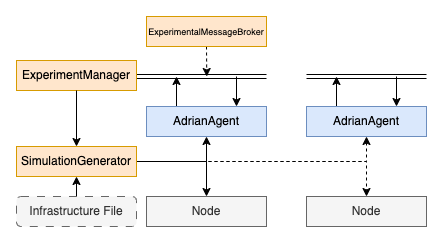
\includegraphics[width=0.8\textwidth]{_content/adrian-experiment-0}
%     \caption{Schematic overview of the baseline experiment, where multiple Agents are disconnected from one another.}
%     \label{fig:baseline}
% \end{figure}
% \comment{Zoltan}{It's not fully clear what this figure conveys. What do the individual symbols mean? In general, it is a good idea to explain all figures in the text, because they are often not as self-explanatory as you might think.}

% \subsection{Experiment 1: Risk Analysis}
% % - Communication, no cooperation
% % - Predefined Infrastructure, same as other experiments
% % - Measure:
% %   - Number of adaptations
% %   - Total number of messages exchanged
% %   - Total number of risks identified
% %   - Number of remaining risks
% %   - Sum of the damage for remaining risks

% The first experiment is conducted to measure the effect of communication between agents. In this experiment agents are able to communicate with each other, \comment{Zoltan}{I think you mean this only for mitigation, not for risk identification?} but are not able to cooperate. 

% When the experiment has started, the agents are allowed to adapt their own properties and software components. The agents are also able to share knowledge at a distance of \( D_{knowledge} \). In this experiment Agents are still not able to cooperate on mitigating risks, which is achieved by not allowing Agents to initiate or join auctions. A simplified overview of the experiment is shown in Figure \ref{fig:experiment-1}.

% \begin{figure}[H]
%     \centering
%     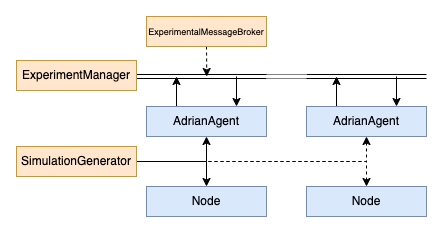
\includegraphics[width=0.8\textwidth]{_content/adrian-experiment-1}
%     \caption{Schematic overview of the first and second experiment, depicting the way multiple Agents are connected to each other and are controlled by the \code{ExperimentManager}.}
%     \label{fig:experiment-1}
% \end{figure}
% \comment{Zoltan}{It's not easy to spot the difference between this and the previous figure, like in a puzzle. Please make the life of your readers easier.}

% This experiment is repeated multiple times, with different values for \( D_{knowledge} \). The values for \( D_{knowledge} \) are 1, 2, and 3. The results of this experiment are compared to the results of the baseline experiment.

% \subsection{Experiment 2: Risk Mitigation}
% % - Communication, cooperation
% % - Predefined Infrastructure, same as other experiments
% % - Measure:
% %   - Number of adaptations
% %   - Total number of messages exchanged
% %   - Total number of risks identified
% %   - Number of remaining risks
% %   - Sum of the damage for remaining risks

% The second experiment is conducted to measure the effect of cooperation between agents. In this experiment agents are able to communicate with each other, and are able to cooperate. 

% When the experiment has started, the agents are allowed to adapt their own properties and software components. The agents are also able to share knowledge at a distance of \( D_{knowledge} \). Additionally, in this experiment Agents are able to cooperate on mitigating risks, which is achieved by allowing Agents to initiate and join auctions. The overview of this experiment is shown in Figure \ref{fig:experiment-1}.

% As with the first experiment, this experiment is repeated multiple times, with different values for \( D_{knowledge} \). The values for \( D_{knowledge} \) are 1, 2, and 3. The results of this experiment are compared to the results of the baseline experiment and the first experiment.
 

\section{Discussion}
\label{sec:discussion}

\begin{figure}[H]
    \centering
    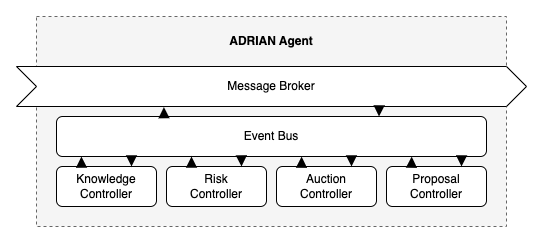
\includegraphics[width=0.8\textwidth]{_content/adrian-component-overview}
    \caption{Agent component overview}
    \label{fig:component-overview}
\end{figure}

\begin{figure}[H]
    \centering
    \includegraphics[width=0.8\textwidth]{_content/knowledge-sharing}
    \caption{Knowledge Exchange Sequence Diagram}
    \label{fig:knowledge-sharing}
\end{figure}


\begin{figure}[H]
    \centering
    \includegraphics[width=1.4\textwidth]{_content/auction}
    \caption{Auction Sequence Diagram}
    \label{fig:auction}
\end{figure}

\section{Future Research}
\label{sec:future-research}

After running the experiments and analyzing the results, we have identified some areas of (potential) improvement in the system. In this section we will discuss some of these areas.

In Section \ref{sssec:knowledge-depth} the concept of knowledge depth was mentioned. As this research kept it at a constant value of 1, it would be interesting to see how this system would perform with different values. This could be done by running the experiments again, but with different values for the knowledge depth. This would give a better understanding of how the knowledge depth affects the performance of the system.

Another area for further research is the risk rules. As mentioned in Section \ref{sssec:risk-rules}, the risk rules are quite simple. It would be interesting to see how the system would perform with more complex risk rules. This could be done by running the experiments again, but with more complex risk rules. This would give a better understanding of how the risk rules affect the performance of the system. 

During the implementation and experimentation some back-and-forth discussions were held about the risk reports that were sent during an auction. The risk reports contain a subsection of the entire attackgraph a node calculated, containing only the nodes that are part of the risk path the auction tries to mitigate. This subsection would contain all risk edges between the nodes, including their probabilities (See figure \ref{fig:riskreport-a}). This would result in a large amount of data being sent during an auction. 

\begin{figure}[H]
    \centering
    \begin{subfigure}[b]{0.4\textwidth}
        \centering
        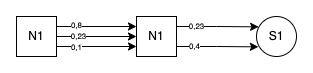
\includegraphics[width=\textwidth]{_content/riskreport-future-research-a.png}
        \caption{Full risk report with all edges.}
        \label{fig:riskreport-a}
    \end{subfigure}
    \hspace{0.5cm}
    \begin{subfigure}[b]{0.4\textwidth}
        \centering
        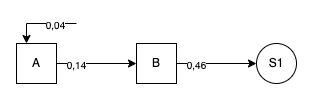
\includegraphics[width=\textwidth]{_content/riskreport-future-research-b.png}
        \caption{Merged risk report with only one edge.}
        \label{fig:riskreport-b}
    \end{subfigure}
    \caption{Two different methods of dealing with risk reports, where on the left all risk edges are present and no information is lost. On the right all risk edges between nodes have been merged into a single edge, resulting in a smaller amount of data being sent.}
\end{figure}


An alternative to sending all edges, was to merge the probabilities of all the edges between two nodes into a single edge (See figure \ref{fig:riskreport-b}). This merging could be done similar to the logic that is used when calculating the risk damage value, for example $p = \prod_{k=1}^{R} (1 - p_{k})$ where $R$ is the risk edges between the nodes, and $p_{k}$ is the probability for an edge. 
This would result in a smaller amount of data being sent during an auction. However, this would also result in a loss of information. Since there are no actual messages sent over the network in the experiments, the amount of data that was sent was not a bottleneck, so the decision was made to send all edges of the subgraph. However, if this system were to be implemented in a real-world scenario, the amount of data sent could be a bottleneck. In that case, it would be interesting to see how the system would perform with the alternative risk report.


\section{Conclusion}
\label{sec:conclusion}

At the start of this research we set out to answer the following research questions:

\vspace{0.5em}
\emph{Can the ADRIAN protocol be implemented and used for effective Risk Assessment and Mitigation?}
\vspace{0.5em}

Which would inturn be answered by the following questions: 
\begin{itemize}
    \item \textit{(Identification) Can we use the ADRIAN protocol to do automated risk identification within a network of nodes with an (imperfect) local knowledge base?}
    \item \textit{(Mitigation) Can the ADRIAN protocol be used to decrease the overall risk, by applying adaptation patterns over time?}
\end{itemize}

In this section we will answer these questions, with the information from the Result and Discussion sections in mind.

\paragraph*{Identification}
In Subsection \ref{ssec:risks-detected} we explained that the full implementation of the ADRIAN protocol is capable of detecting risks in a network of nodes. By using an internal knowledge base agents are able to detect risks that they would otherwise be unable to detect. The benefits of this decentralized approach are that agents only need to store, share, and assess the properties of each node for a subset of the problem. This makes it very scalable and allows for a large number of nodes to be added to the network. However, this also means that the agents are unable to detect risks that are outside of their knowledge base. This is a trade-off that is made in the ADRIAN protocol. 

\paragraph*{Mitigation}
The ADRIAN protocol, even without auctions, is able to decrease the overall risk and predicted damage of an infrastructure.
Subsections \ref{ssec:efficient-adaptations} and \ref{ssec:adaptation-time} explain that the full implementation of the ADRIAN protocol is capable of reducing the overall damage of the infrastructure, by using the concepts of auctions. These auctions allow agents to apply more effective adaptations, and reduce the amount of service-/downtime a node and its software components experience. 


\vspace{0.5em}
Combining all the information from Section \ref{sec:discussion} and the answers to the sub-research questions, we can conclude that the ADRIAN protocol can be used for effective risk assessment and mitigation. 


\bibliographystyle{abbrv}
\bibliography{bibliography}
\end{document}
